\chapter{Số tự nhiên, Số nguyên và Số hữu tỉ}\label{chapter4:natural-numbers-integers-and-rationals}

\noindent ``God made the natural numbers; all else is the work of man.\@''

\noindent \rule[0.5ex]{2cm}{0.5pt}

\noindent \textit{Leopold Kronecker ($1823-1891$)}

\section{Hệ tiên đề Peano về các số tự nhiên}

\subsection*{Hệ tiên đề Peano}

Cuối thế kỉ 19, nhà toán học người Ý Giuseppe Peano đưa ra một hệ tiên đề về các số tự nhiên. Hệ tiên đề này gồm 9 tiên đề sau.

\begin{axiom}
	$0$ và $S$ là hai đối tượng không được định nghĩa.

	\begin{enumerate}[label={(PA\arabic*)},itemsep=0pt,topsep=0pt,itemindent=0.25cm]
		\item $0$ là một số tự nhiên.
		\item Với mọi số tự nhiên $x$, có $x = x$.
		\item Với mọi số tự nhiên $x$ và $y$, nếu $x = y$ thì $y = x$.
		\item Với mọi số tự nhiên $x, y$, và $z$, nếu $x = y$ và $y = z$ thì $x = z$.
		\item Với mọi $x$ và $y$, nếu $y$ là số tự nhiên và $x = y$ thì $x$ cũng là một số tự nhiên.
		\item Với mọi số tự nhiên $x$, $S(x)$ là một số tự nhiên.
		\item Với mọi số tự nhiên $x$ và $y$, nếu $S(x) = S(y)$ thì $x = y$.
		\item Với mọi số tự nhiên $x$, $S(x) \ne 0$.
		\item Nếu một tập hợp $A$ thỏa mãn hai điều kiện sau
		      \begin{itemize}[itemsep=0pt,topsep=0pt]
			      \item $0\in A$,
			      \item với mọi số tự nhiên $n$, $n\in A$ kéo theo $S(n)\in A$,
		      \end{itemize}
		      thì mọi số tự nhiên đều thuộc $A$.
	\end{enumerate}
\end{axiom}

Tập hợp (tất cả) các số tự nhiên được kí hiệu là $\mathbb{N}$.

Tiên đề 1 khẳng định tập hợp số tự nhiên không rỗng. Hệ tiên đề ban đầu của Peano chọn $1$ làm số tự nhiên ``đầu tiên'' thay vì $0$. Nhưng trong tác phẩm chính thức của mình, ông lại chọn số $0$ làm số tự nhiên đầu tiên. Cho đến nay, cộng đồng toán học không thống nhất rằng $0$ là số tự nhiên hay không $-$ Đây chỉ là vấn đề quy ước. Vì sự nhập nhằng đó, thay vì viết là ``số tự nhiên'', nhiều tác giả chọn cách viết là ``số nguyên dương'', ``số nguyên không âm''.

Tiên đề 2, 3, 4, 5 nói về quan hệ bằng nhau trên tập hợp số tự nhiên. Ba tiên đề 2, 3, 4 khẳng định quan hệ bằng nhau trên tập hợp số tự nhiên là một quan hệ tương đương. Tiên đề 5 có nghĩa là tập hợp số tự nhiên là \textit{đóng} dưới quan hệ bằng nhau (một số tự nhiên không thể bằng một đối tượng nào đó nằm ngoài tập hợp số tự nhiên).

Đối tượng $S$ không được định nghĩa trong hệ tiên đề trên. $S$ được gọi là hàm successor (có nghĩa là kế tiếp, chúng tôi không dùng tên gọi được dịch). Tiên đề 6 phát biểu rằng tập hợp số tự nhiên đóng dưới hàm successor. Tiên đề 7 có nghĩa là $S$ là một đơn ánh. Tiên đề 8 có nghĩa là không có số tự nhiên nào nhận $0$ làm số tự nhiên liền sau nó. Ý nghĩa của hàm successor là nó gán một số tự nhiên với số tự nhiên ngay kế tiếp.

Tiên đề 9 chính là nguyên lý quy nạp toán học. Tiên đề 9 còn được gọi là \textit{tiên đề quy nạp}.

Ở mục tiếp theo, chúng ta sẽ định nghĩa phép cộng, phép nhân, quan hệ thứ tự trên tập hợp số tự nhiên, và chứng minh nhiều tính chất của chúng. Bên cạnh 9 tiên đề Peano, hai công cụ duy nhất chúng ta có là phương pháp phản chứng và phương pháp quy nạp toán học. Do đó, ở hai mục tiếp theo, phương pháp quy nạp toán học sẽ được áp dụng triệt để. Dưới đây là chứng minh cho nguyên lý quy nạp toán học.

Chúng ta nhắc lại nội dung nguyên lý quy nạp toán học: Nếu hai điều kiện sau thỏa mãn
\begin{enumerate}[label={(\roman*)}]
	\item mệnh đề $p(0)$ đúng,
	\item với mọi số tự nhiên $k\geq 0$, $p(k)$ kéo theo $p(k+1)$,
\end{enumerate}

thì $p(n)$ đúng với mọi số tự nhiên $n$.

\begin{proof}[Chứng minh nguyên lý quy nạp toán học]
	Chúng ta gọi $A$ là tập hợp các số tự nhiên $n$ sao cho có $p(n)$.

	Vì có $p(0)$ nên $0\in A$.

	Vì với mọi số tự nhiên $k\geq 1$, $p(k)$ kéo theo $p(k+1)$ nên với mọi số tự nhiên $k\geq 1$, $k\in A$ kéo theo $(k+1)\in A$.

	Theo tiên đề 9, $A$ chứa mọi số tự nhiên. Theo định nghĩa của tập hợp $A$, có $p(n)$ với mọi số tự nhiên $n$.
\end{proof}

Có thể bạn đọc đã bỏ qua một câu hỏi: ``Ngoài $0$, còn số tự nhiên $n$ nào mà không tồn tại số tự nhiên $m$ sao cho $S(m) = n$ không?\@'' Câu trả lời là không. Nhưng chúng ta cần một chứng minh.
\begin{theorem}\label{theorem:successor}
	Nếu $n$ là một số tự nhiên khác $0$ thì tồn tại một số tự nhiên $m$ sao cho $S(m) = n$.
\end{theorem}

\begin{proof}
	Mệnh đề có phát biểu tương đương như sau: Với mọi số tự nhiên $n$, nếu $n$ khác $0$ thì tồn tại số tự nhiên $m$ sao cho $S(m) = n$.

	Khi $n = 0$, tức là mệnh đề $n$ là số tự nhiên khác $0$ sai, thì theo tiên đề 8 không có số tự nhiên $m$ nào sao cho $S(m) = n$ (lưu ý rằng mệnh đề kéo theo $P\implies Q$ đúng khi $P$ và $Q$ sai).

	Khi $n = 1$, chúng ta có $S(0) = 1$.

	Giả sử với số tự nhiên $k\geq 1$, $n = k$ kéo theo tồn tại số tự nhiên $m$ sao cho $S(m) = k$. Khi đó $S(S(m)) = S(k)$.

	Theo nguyên lý quy nạp toán học, với mọi số tự nhiên $n$ khác không, tồn tại số tự nhiên $m$ sao cho $S(m) = n$.
\end{proof}

Hệ quả của định lý trên là tập hợp số tự nhiên bao gồm các phần tử sau (Hình~\ref{fig:first-five-natural-numbers}).
\begin{figure}[htp]
	\centering
	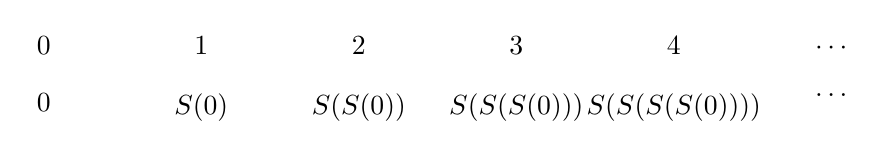
\begin{tikzpicture}
		\coordinate (number0) at (0,0);
		\coordinate (number1) at (2cm,0);
		\coordinate (number2) at (4cm,0);
		\coordinate (number3) at (6cm,0);
		\coordinate (number4) at (8cm,0);
		\coordinate (etc) at (10cm,0);

		\node[label={[black]above:$0$},label={[black]below:$0$}] at (number0) {};
		\node[label={[black]above:$1$},label={[black]below:$S(0)$}] at (number1) {};
		\node[label={[black]above:$2$},label={[black]below:$S(S(0))$}] at (number2) {};
		\node[label={[black]above:$3$},label={[black]below:$S(S(S(0)))$}] at (number3) {};
		\node[label={[black]above:$4$},label={[black]below:$S(S(S(S(0))))$}] at (number4) {};
		\node[label={[black]above:$\cdots$},label={[black]below:$\ldots$}] at (etc) {};
	\end{tikzpicture}
    \caption{Năm phần tử đầu tiên của tập hợp số tự nhiên theo hệ tiên đề Peano.}\label{fig:first-five-natural-numbers}
\end{figure}

Ý niệm và kí hiệu cho các số tự nhiên được xuất hiện trước hệ tiên đề của Peano hàng nghìn năm. Các kí hiệu (các số) $1, 2, 3,\ldots$ lần lượt chính là $S(0), S(S(0)), S(S(S(0))),\ldots$

Chúng tôi muốn nhấn mạnh một lần nữa: trong hai mục tiếp theo, chúng ta sẽ áp dụng liên tục phương pháp quy nạp toán học.

\subsection*{Các phép toán số học trên tập hợp số tự nhiên}

Bạn đọc không cần quá chú ý tới kĩ thuật chứng minh trong mục này. Tuy nhiên, chúng tôi cung cấp chứng minh chậm rãi và chi tiết cho mục đích tham khảo. Luận cho cùng, mọi thứ được xây dựng từ các số tự nhiên.

Hai phép toán cơ bản với số tự nhiên là phép cộng và phép nhân. Trong mục này, chúng ta sẽ định nghĩa hai phép toán cộng và nhân trên tập hợp số tự nhiên theo hệ tiên đề Peano, sau đó chứng minh các tính chất cơ bản của chúng.

Phép cộng hai số tự nhiên được định nghĩa bằng đệ quy như sau.

\begin{definition}[Phép cộng]
	Cho $x$ và $y$ là hai số tự nhiên. Phép cộng hai số tự nhiên là một phép toán hai ngôi trên $\mathbb{N}$, kí hiệu là $+$. Chúng ta định nghĩa
	\[
		x + 0 = x\qquad\text{và}\qquad x + S(y) = S(x + y).
	\]
\end{definition}

Nhằm minh họa cho định nghĩa này, chúng ta làm một vài phép cộng.
\begin{example}
	Cho số tự nhiên $x$.
	\begin{align*}
		 & x + 0 = x,                                      \\
		 & x + S(0) = S(x + 0) = S(x),                     \\
		 & x + S(1) = x + S(S(0)) = S(x + S(0)) = S(S(x)).
	\end{align*}
\end{example}

Chúng ta sử dụng nguyên lý quy nạp toán học để chứng minh hai tính chất kết hợp và tính chất giao hoán của phép cộng hai số tự nhiên.
\begin{theorem}
	Trên tập hợp số tự nhiên
	\begin{enumerate}[label={(\roman*)}]
		\item Phép cộng có tính chất kết hợp. Tức là, với mọi số tự nhiên $x, y, z$, chúng ta có $(x + y) + z = x + (y + z)$. Bằng kí hiệu logic hình thức, chúng ta viết
		      \[
			      \forall x\forall y\forall z \left( (x + y) + z = x + (y + z) \right).
		      \]
		\item Với mọi số tự nhiên $x$, có $0 + x = x$.
		\item Phép cộng có tính chất giao hoán.  Tức là, với mọi số tự nhiên $x, y$, chúng ta có $x + y = y + x$. Bằng kí hiệu logic hình thức, chúng ta viết
		      \[
			      \forall x\forall y \left( x + y = y + x \right).
		      \]
	\end{enumerate}
\end{theorem}

\begin{proof}
	\begin{enumerate}[label={(\roman*)}]
		\item Nếu $z = 0$ thì $(x + y) + z = x + y = x + (y + 0) = x + (y + z)$.

		      Giả sử với số tự nhiên $z = n$, $(x + y) + n = x + (y + n)$. Chúng ta sẽ chứng minh $(x + y) + S(n) = x + (y + S(n))$.
		      \begin{align*}
			      (x + y) + S(n) & = S((x + y) + n)  & \text{(theo định nghĩa phép cộng trên $\mathbb{N}$)} \\
			                     & = S(x + (y + n))  & \text{(theo giả thiết quy nạp)}                      \\
			                     & = x + S(y + n)    & \text{(theo định nghĩa phép cộng trên $\mathbb{N}$)} \\
			                     & = x + (y + S(n)). & \text{(theo định nghĩa phép cộng trên $\mathbb{N}$)}
		      \end{align*}

		      Vậy theo nguyên lý quy nạp toán học, $(x + y) + z = x + (y + z)$ với mọi số tự nhiên $x, y, z$.
		\item Khi $x = 0$, $0 + 0 = 0$, theo định nghĩa phép cộng trên tập hợp số tự nhiên.

		      Giả sử với số tự nhiên $x = n$, $0 + n = n$. Khi đó
		      \begin{align*}
			      0 + S(n) & = S(0 + n) & \text{(theo định nghĩa phép cộng trên $\mathbb{N}$)} \\
			               & = S(n).    & \text{(theo giả thiết quy nạp)}
		      \end{align*}

		      Theo nguyên lý quy nạp toán học, $0 + x = x$ với mọi số tự nhiên $x$.
		\item Khi $y = 0$ thì $x + 0 = x = 0 + x$, theo định nghĩa phép cộng hai số tự nhiên và phần (ii).

		      Chúng tôi gặp khó khăn khi cố gắng chứng minh tính chất giao hoán của phép cộng hai số tự nhiên bằng \textit{một lần} quy nạp. Trước hết, chúng ta chứng minh mệnh đề sau: $x + S(0) = S(0) + x$ với mọi số tự nhiên $x$.

		      Khi $x = 0$, theo định nghĩa phép cộng hai số tự nhiên, $0 + S(0) = S(0 + 0) = S(0) = S(0) + 0$.

		      Giả sử với số tự nhiên $x = n$, có $n + S(0) = S(0) + n$. Khi đó
		      \begin{align*}
			      S(0) + S(n) & = S(S(0) + n)  & \text{(theo định nghĩa phép cộng trên $\mathbb{N}$)} \\
			                  & = S(n + S(0))  & \text{(theo giả thiết quy nạp)}                      \\
			                  & = S(S(n))      & \text{(theo định nghĩa phép cộng trên $\mathbb{N}$)} \\
			                  & = S(S(n) + 0)  & \text{(theo định nghĩa phép cộng trên $\mathbb{N}$)} \\
			                  & = S(n) + S(0). & \text{(theo định nghĩa phép cộng trên $\mathbb{N}$)}
		      \end{align*}

		      Theo nguyên lý quy nạp toán học, $x + S(0) = S(0) + x$ với mọi số tự nhiên $x$.

		      Chúng ta thực hiện chứng minh bằng quy nạp một lần nữa cho mệnh đề $x + y = y + x$ với mọi số tự nhiên $x, y$.

		      Khi $y = 0$ và khi $y = S(0)$, chúng ta lần lượt có $x + 0 = x = 0 + x$ (theo phần (ii)) và $x + S(0) = S(0) + x$ (theo mệnh đề vừa chứng minh).

		      Giả sử với số tự nhiên $y = n$, $x + n = n + x$. Khi đó
		      \begin{align*}
			      x + S(n) & = S(x + n)       & \text{(theo định nghĩa phép cộng trên $\mathbb{N}$)} \\
			               & = S(n + x)       & \text{(theo giả thiết quy nạp)}                      \\
			               & = S((n + x) + 0) & \text{(theo định nghĩa phép cộng trên $\mathbb{N}$)} \\
			               & = (n + x) + S(0) & \text{(theo định nghĩa phép cộng trên $\mathbb{N}$)} \\
			               & = S(0) + (n + x) & \text{(theo mệnh đề vừa chứng minh)}                 \\
			               & = (S(0) + n) + x & \text{(theo phần (i))}                               \\
			               & = (n + S(0)) + x & \text{(theo mệnh đề vừa chứng minh)}                 \\
			               & = S(n) + x.      & \text{(theo định nghĩa phép cộng trên $\mathbb{N}$)}
		      \end{align*}

		      Theo nguyên lý quy nạp toán học, $x + y = y + x$ với mọi số tự nhiên $x, y$.
	\end{enumerate}
\end{proof}

Phép nhân cũng được định nghĩa bằng đệ quy.
\begin{definition}[Phép nhân]
	Cho $x$ và $y$ là hai số tự nhiên. Phép nhân hai số tự nhiên là một phép toán hai ngôi trên $\mathbb{N}$, kí hiệu là $\cdot$. Chúng ta định nghĩa
	\[
		x\cdot 0 = 0\qquad\text{và}\qquad x\cdot S(y) = x + (x\cdot y).
	\]
\end{definition}

Tương tự, chúng ta làm một vài phép nhân với định nghĩa này.

\begin{example}
	Cho số tự nhiên $x$.
	\begin{align*}
		 & x \cdot 0 = 0,                                                                 \\
		 & x \cdot 1 = x\cdot S(0) = x + (x\cdot 0) = x + 0 = x,                          \\
		 & x \cdot 2 = x\cdot S(S(0)) = x + (x\cdot S(0)) = x + (x + (x\cdot 0)) = x + x.
	\end{align*}
\end{example}

Chúng ta nhắc lại và chứng minh các tính chất sau của phép nhân hai số tự nhiên.

\begin{theorem}
	Trên tập hợp số tự nhiên
	\begin{enumerate}[label={(\roman*)}]
		\item Phép nhân có tính chất phân phối (từ bên phải) với phép cộng. Tức là, với mọi số tự nhiên $x, y, z$, chúng ta có $(x + y)\cdot z = (x\cdot z) + (y\cdot z)$.
		\item Phép nhân có tính chất kết hợp. Tức là, với mọi số tự nhiên $x, y, z$, chúng ta có $(x \cdot y) \cdot z = x \cdot (y \cdot z)$. Bằng kí hiệu logic hình thức, chúng ta viết
		      \[
			      \forall x\forall y\forall z \left( (x \cdot y) \cdot z = x \cdot (y \cdot z) \right).
		      \]
		\item Với mọi só tự nhiên $x$, $0\cdot x = 0$.
		\item Với mọi số tự nhiên $x$, $x\cdot S(0) = S(0) \cdot x = x$.
		\item Phép nhân có tính chất giao hoán.  Tức là, với mọi số tự nhiên $x, y$, chúng ta có $x \cdot y = y \cdot x$. Bằng kí hiệu logic hình thức, chúng ta viết
		      \[
			      \forall x\forall y \left( x \cdot y = y \cdot x \right).
		      \]
	\end{enumerate}
\end{theorem}

\begin{proof}
	\begin{enumerate}[label={(\roman*)}]
		\item Nếu $z = 0$ thì theo định nghĩa phép nhân và phép cộng hai số tự nhiên
		      \begin{align*}
			      (x + y)\cdot z & = (x + y)\cdot 0 = 0 = 0 + 0 = (x\cdot 0) + (y\cdot 0) = (x\cdot z) + (y\cdot z).
		      \end{align*}

		      Giả sử với $z = n$, có $(x + y)\cdot n = (x\cdot n) + (y\cdot n)$. Khi đó
		      \begin{align*}
			      (x + y)\cdot S(n) & = (x + y) + (x + y)\cdot n            & \text{(theo định nghĩa phép nhân trên $\mathbb{N}$)}              \\
			                        & = (x + y) + ((x\cdot n) + (y\cdot n)) & \text{(theo giả thiết quy nạp)}                                   \\
			                        & = ((x + y) + (x\cdot n)) + (y\cdot n) & \text{(theo tính chất kết hợp của phép cộng trên $\mathbb{N}$)}   \\
			                        & = (x + (y + (x\cdot n))) + (y\cdot n) & \text{(theo tính chất kết hợp của phép cộng trên $\mathbb{N}$)}   \\
			                        & = (x + ((x\cdot n) + y)) + (y\cdot n) & \text{(theo tính chất giao hoán của phép cộng trên $\mathbb{N}$)} \\
			                        & = ((x + (x\cdot n)) + y) + (y\cdot n) & \text{(theo tính chất kết hợp của phép cộng trên $\mathbb{N}$)}   \\
			                        & = (x + (x\cdot n)) + (y + (y\cdot n)) & \text{(theo tính chất kết hợp của phép cộng trên $\mathbb{N}$)}   \\
			                        & = (x\cdot S(n)) + (y\cdot S(n)).      & \text{(theo định nghĩa của phép nhân trên $\mathbb{N}$)}
		      \end{align*}

		      Theo nguyên lý quy nạp toán học, $(x + y)\cdot z = (x\cdot z) + (y\cdot z)$ với mọi số tự nhiên $x, y, z$.
		\item Nếu $z = 0$ thì theo định nghĩa phép nhân hai số tự nhiên, $(x\cdot y)\cdot z = 0 = x\cdot 0 = x\cdot (y\cdot 0) = x\cdot (y\cdot z)$.

		      Giả sử với số tự nhiên $z = n$, có $(x\cdot y)\cdot n = x\cdot (y\cdot n)$. Khi đó
		      \begin{align*}
			      (x\cdot y)\cdot S(n) & = (x\cdot y) + ((x\cdot y)\cdot n) & \text{(theo định nghĩa phép nhân trên $\mathbb{N}$)}            \\
			                           & = (x\cdot y) + (x\cdot (y\cdot n)) & \text{(theo tính chất kết hợp của phép nhân trên $\mathbb{N}$)} \\
			                           & = x\cdot (y + (y\cdot n))          & \text{(theo phần (i))}                                          \\
			                           & = x\cdot (y\cdot S(n)).            & \text{(theo định nghĩa phép nhân trên $\mathbb{N}$)}
		      \end{align*}

		      Theo nguyên lý quy nạp toán học, $(x\cdot y)\cdot z = x\cdot (y\cdot z)$ với mọi số tự nhiên $x, y, z$.
		\item Khi $x = 0$, chúng ta có $0\cdot x = 0\cdot 0 = 0$, theo định nghĩa phép nhân trên tập số tự nhiên.

		      Giả sử với $x = n$, chúng ta có $0\cdot n = 0$. Khi đó
		      \begin{align*}
			      0\cdot S(n) & = 0 + (0\cdot n) & \text{(theo định nghĩa phép nhân trên $\mathbb{N}$)} \\
			                  & = 0 + 0          & \text{(theo giả thiết quy nạp)}                      \\
			                  & = 0.             & \text{(theo định nghĩa phép cộng trên $\mathbb{N}$)}
		      \end{align*}

		      Theo nguyên lý quy nạp toán học, $0\cdot x = 0$ với mọi số tự nhiên $x$.
		\item Theo định nghĩa phép nhân và phép cộng hai số tự nhiên, $x\cdot S(0) = x + (x\cdot 0) = x + 0 = x$.

		      Chúng ta cần chứng minh $S(0)\cdot x = x$ với mọi số tự nhiên $x$. Khi $x = 0$, chúng ta có $S(0)\cdot 0 = 0$, theo định nghĩa của phép nhân hai số tự nhiên.

		      Giả sử với số tự nhiên $x = n$, chúng ta có $S(0)\cdot n = n$. Khi đó
		      \begin{align*}
			      S(0)\cdot S(n) & = S(0) + (S(0)\cdot n) & \text{(theo định nghĩa của phép nhân trên $\mathbb{N}$)}          \\
			                     & = S(0) + n             & \text{(theo giả thiết quy nạp)}                                   \\
			                     & = n + S(0)             & \text{(theo tính chất giao hoán của phép cộng trên $\mathbb{N}$)} \\
			                     & = S(n).                & \text{(theo định nghĩa của phép cộng trên $\mathbb{N}$)}
		      \end{align*}

		      Theo nguyên lý quy nạp toán học, $x\cdot S(0) = S(0)\cdot x = x$ với mọi số tự nhiên $x$.
		\item Khi $y = 0$, theo định nghĩa phép nhân trên tập hợp số tự nhiên và phần (iii), chúng ta có $x\cdot 0 = 0\cdot x = 0$.

		      Giả sử với số tự nhiên $y = n$, chúng ta có $x\cdot n = n\cdot x$. Khi đó
		      \begin{align*}
			      x\cdot S(n) & = x + (x\cdot n)             & \text{(định nghĩa phép nhân trên $\mathbb{N}$)}                   \\
			                  & = x + (n\cdot x)             & \text{(theo giả thiết quy nạp)}                                   \\
			                  & = (S(0)\cdot x) + (n\cdot x) & \text{(theo phần (iv))}                                           \\
			                  & = (S(0) + n)\cdot x          & \text{(theo phần (i))}                                            \\
			                  & = (n + S(0))\cdot x          & \text{(theo tính chất giao hoán của phép cộng trên $\mathbb{N}$)} \\
			                  & = S(n)\cdot x.               & \text{(theo định nghĩa phép cộng trên $\mathbb{N}$)}
		      \end{align*}

		      Theo nguyên lý quy nạp toán học, $x\cdot y = y\cdot x$ với mọi số tự nhiên $x, y$.
	\end{enumerate}
\end{proof}

Với những tính chất đã chứng minh của phép cộng và phép nhân hai số tự nhiên, chúng ta rút ra hệ quả sau.

\begin{corollary}
	Trên tập hợp số tự nhiên, phép nhân có tính chất phân phối với phép cộng (từ cả hai phía). Bằng kí hiệu, điều này nghĩa là với mọi số tự nhiên $x, y, z$, chúng ta có
	\[
		\begin{split}
			(x + y)\cdot z = (x\cdot z) + (y\cdot z), \\
			z\cdot (x + y) = (z\cdot x) + (z\cdot y).
		\end{split}
	\]
\end{corollary}

Chúng ta khép lại nội dung về phép cộng và phép nhân trên tập số tự nhiên bằng một lưu ý. Thói quen học tập, tính toán, và cả các chứng minh trong mục này có thể gây ra một ấn tượng \textit{không chính xác} rằng tính chất kết hợp và tính chất giao hoán luôn song hành. Thực tế, khi học và làm toán, chúng ta sẽ bắt gặp những phép toán trên những tập hợp nhất định mà \textit{không có tính chất kết hợp lẫn giao hoán}, hoặc \textit{có tính chất giao hoán nhưng không có tính chất kết hợp}, hoặc \textit{có tính chất kết hợp mà không có tính chất giao hoán} (chẳng hạn như phép toán hợp thành hai ánh xạ).

\subsection*{Quan hệ thứ tự trên tập hợp số tự nhiên}

Số tự nhiên đã trở nên quá quen thuộc với chúng ta, đến nỗi việc nói rằng số này bé hơn số kia được coi là hiển nhiên. Tuy nhiên, để học và làm toán, chúng ta vẫn cần những định nghĩa hình thức tương thích với hệ tiên đề và những định lý mà chúng ta sử dụng.

\begin{definition}[Quan hệ thứ tự trên tập hợp số tự nhiên]
	Số tự nhiên $x$ được gọi là nhỏ hơn hoặc bằng số tự nhiên $y$ nếu và chỉ nếu tồn tại số tự nhiên $z$ sao cho $x + z = y$. Khi đó, chúng ta kí hiệu $x\leq y$. Nếu $x\leq y$ và $x\ne y$ thì chúng ta nói $x$ nhỏ hơn $y$ và kí hiệu $x < y$.
\end{definition}

Dựa trên định nghĩa này, chúng ta vẫn phải kiểm tra quan hệ nhỏ hơn hoặc bằng trên tập hợp số tự nhiên có thỏa mãn ba tính chất của quan hệ thứ tự hay không. Tuy nhiên, việc chứng minh tính chất phản đối xứng tỏ ra khó khăn hơn cả.

\begin{proposition}
	Chứng minh rằng
	\begin{enumerate}[label={(\roman*)}]
		\item Quan hệ $\leq$ trên tập hợp số tự nhiên thỏa mãn tính chất phản xạ và bắc cầu.
		\item Với mọi số tự nhiên $x$, có $x\ne S(x)$.
		\item Nếu hai số tự nhiên $x$ và $y$ thỏa mãn $x + y = x$ thì $y = 0$.
		\item Hai số tự nhiên $a$ và $b$ thỏa mãn $a + b = 0$ khi và chỉ khi $a = b = 0$.
		\item Quan hệ $\leq$ trên tập hợp số tự nhiên thỏa mãn tính chất phản đối xứng.
		\item Quan hệ $\leq$ trên tập hợp số tự nhiên là một quan hệ thứ tự toàn phần.
	\end{enumerate}
\end{proposition}

\begin{proof}
	\begin{enumerate}[label={(\roman*)}]
		\item Với mọi số tự nhiên, chúng ta có $x + 0 = x$. Do đó $x\leq x$. Như vậy quan hệ $\leq$ trên tập hợp số tự nhiên có tính chất phản xạ.

		      Nếu ba số tự nhiên $x, y, z$ thỏa mãn $x\leq y$ và $y\leq z$ thì theo định nghĩa của $\leq$, tồn tại các số tự nhiên $m$ và $n$ sao cho $x + m = y$ và $y + n = z$. Khi đó
		      \begin{align*}
			      z & = y + n       \\
			        & = (x + m) + n \\
			        & = x + (m + n)
		      \end{align*}

		      Theo định nghĩa của $\leq$, chúng ta suy ra $x\leq z$. Như vậy quan hệ $\leq$ trên tập hợp số tự nhiên có tính chất bắc cầu.
		\item Khi $x = 0$, $0\ne S(0)$ theo tiên đề 8.

		      Giả sử với số tự nhiên $x = n$, có $n\ne S(n)$. Theo giả thiết quy nạp và tiên đề 7, $S(n)\ne S(S(n))$.

		      Vậy theo nguyên lý quy nạp toán học, $x\ne S(x)$ với mọi số tự nhiên $x$.
		\item Chúng ta nhìn mệnh đề cần chứng minh theo quan điểm khác để chứng minh bằng quy nạp toán học: Với mọi số tự nhiên $x$, $x + y = x$ kéo theo $y = 0$.

		      Khi $x = 0$ thì $y = 0 + y = 0$. Giả sử với $x = n$, chúng ta có ``$n + y = n$ kéo theo $y = 0$''. Khi đó, nếu $S(n) + y = S(n)$ thì
		      \begin{align*}
			      S(n + y) & = S(y + n) & \text{(theo tính chất giao hoán của phép cộng trên $\mathbb{N}$)} \\
			               & = y + S(n) & \text{(theo định nghĩa phép cộng trên $\mathbb{N}$)}              \\
			               & = S(n) + y & \text{(theo tính chất giao hoán của phép cộng trên $\mathbb{N}$)} \\
			               & = S(n).
		      \end{align*}

		      Từ đẳng thức $S(n + y) = S(n)$, theo tiên đề 7, chúng ta có $n + y = n$. Theo giả thiết quy nạp, $y = 0$. Do đó $S(n) + y = S(n)$ kéo theo $y = 0$. Như vậy, theo nguyên lý quy nạp, với mọi số tự nhiên $x$, $x + y = x$ kéo theo $y = 0$.

		      Vậy khi hai số tự nhiên $x, y$ thỏa mãn $x + y = x$ thì $y = 0$.
		\item ($\Rightarrow$) $a = b = 0$.

		      Theo định nghĩa phép cộng trên tập hợp số tự nhiên, $a + b = 0 + 0 = 0$.

		      ($\Leftarrow$) $a + b = 0$.

		      Giả sử phản chứng rằng $a\ne 0$. Khi đó tồn tại số tự nhiên $c$ sao cho $S(c) = a$. Theo định nghĩa phép cộng hai số tự nhiên và tính chất giao hoán của phép cộng hai số tự nhiên, chúng ta có $0 = b + a = b + S(c) = S(b + c)$. Điều này mâu thuẫn với tiên đề 8. Do đó $a = 0$.

		      Tương tự, cũng bằng phương pháp phản chứng, chúng ta chỉ ra được $b = 0$.

		      Vậy hai số tự nhiên $a, b$ thỏa mãn $a + b = 0$ khi và chỉ khi $a = b = 0$.
		\item Nếu hai số tự nhiên $x$ và $y$ thỏa mãn $x\leq y$ và $y\leq x$ thì theo định nghĩa quan hệ $\leq$ trên tập hợp số tự nhiên, tồn tại hai số tự nhiên $a$ và $b$ sao cho $x + a = y$ và $y + b = x$. Khi đó
		      \begin{align*}
			      x & = y + b                                                                         \\
			        & = (x + a) + b                                                                   \\
			        & = x + (a + b) & \text{(theo tính chất kết hợp của phép cộng trên $\mathbb{N}$)}
		      \end{align*}

		      Theo phần (iii) và (iv), chúng ta kết luận $a = b = 0$, dẫn tới $x = y$. Như vậy, quan hệ $\leq$ trên tập hợp số tự nhiên có tính chất phản đối xứng.
		\item Phần (i) và (v) khẳng định rằng quan hệ $\leq$ trên tập hợp số tự nhiên là một quan hệ thứ tự.

		      Để chứng minh quan hệ $\leq$ trên tập hợp số tự nhiên là quan hệ thứ tự toàn phần, chúng ta chứng minh: Với mọi số tự nhiên $x, y$, có $x\leq y$ hoặc $y\leq x$.

		      Đầu tiên, với mọi số tự nhiên $x$, có $0\leq x$ hoặc $x\leq 0$. Giả sử với số tự nhiên $y = n$, với mọi số tự nhiên $x$, có $n\leq x$ hoặc $x\leq n$. Sử dụng giả thiết quy nạp, chúng ta xem xét hai trường hợp sau.

              Trường hợp $x\leq n$. Theo định nghĩa phép cộng hai số tự nhiên, $n + S(0) = S(n)$ nên $n\leq S(n)$ theo định nghĩa quan hệ $\leq$ trên tập hợp số tự nhiên. Từ tính chất bắc cầu của quan hệ $\leq$ trên tập hợp số tự nhiên, chúng ta suy ra $x\leq S(n)$.

              Trường hợp $n\leq x$. Theo định nghĩa quan hệ thứ tự trên tập hợp số tự nhiên, tồn tại số tự nhiên $a$ sao cho $n + a = x$. Nếu $x = n$ thì $x\leq S(n)$ vì $n\leq S(n)$ (rút ra từ phần chứng minh của trường hợp trên). Còn nếu $n < x$ thì $a$ khác không (theo phần (ii)). Theo Định lý~\ref{theorem:successor}, vì $a$ khác không nên tồn tại số tự nhiên $b$ sao cho $a = S(b)$. Theo định nghĩa phép cộng hai số tự nhiên, $x = n + a = n + S(b) = S(n + b)$. Bên cạnh đó, $S(n) + b = b + S(n) = S(b + n) = S(n + b) = x$, nên theo định nghĩa quan hệ $\leq$ trên tập hợp số tự nhiên, chúng ta có $S(n)\leq x$.

              Tóm lại, từ cả hai trường hợp, chúng ta kết luận: với mọi số tự nhiên $x$, $x\leq S(n)$ hoặc $S(n)\leq x$. Theo nguyên lý quy nạp, với mọi cặp số tự nhiên $x$ và $y$, có $x\leq y$ hoặc $y\leq x$.

              Vậy quan hệ $\leq$ trên tập hợp số tự nhiên là một quan hệ thứ tự toàn phần.\qedhere
	\end{enumerate}
\end{proof}

\section{Số nguyên}

\subsection*{Phép trừ hai số tự nhiên}

\subsection*{Tập hợp số nguyên}

\subsection*{Các phép toán và quan hệ trên tập số nguyên}

\section{Nguyên lý quy nạp toán học}

\subsection*{Nguyên lý quy nạp toán học và nguyên lý quy nạp mạnh}

\subsection*{Nguyên lý thứ tự tốt}

\subsection*{$\dagger$ Nguyên lý quy nạp Cauchy}

\subsection*{$\dagger$ Giảm vô hạn}

\section{Số hữu tỉ}

\subsection*{Phép chia hai số tự nhiên, hai số nguyên}

\subsection*{Tập hợp số hữu tỉ}

\subsection*{Các phép toán và quan hệ trên tập số hữu tỉ}
